\documentclass[%
12pt,
master,  % тип документа
natbib,      % использовать пакет natbib для "сжатия" цитирований
subf,        % использовать пакет subcaption для вложенной нумерации рисунков
substylefile = spbu.rtx,
href,        % использовать пакет hyperref для создания гиперссылок
colorlinks,  % цветные гиперссылки
%fixint,     % включить прямые знаки интегралов
]{disser}

\usepackage[
  a4paper, mag=1000,
  left=2.5cm, right=1cm, top=2cm, bottom=2cm, headsep=0.7cm, footskip=1cm
]{geometry}


\usepackage[colorinlistoftodos]{todonotes}

\usepackage[intlimits]{amsmath}
\usepackage{amssymb,amsfonts}

\usepackage[T2A]{fontenc}
\usepackage[utf8]{inputenc}
\usepackage[english,russian]{babel}
\ifpdf\usepackage{epstopdf}\fi
\usepackage[autostyle]{csquotes}

% Шрифт Times в тексте как основной
%\usepackage{tempora}
% альтернативный пакет из дистрибутива TeX Live
%\usepackage{cyrtimes}

% Шрифт Times в формулах как основной
%\usepackage[varg,cmbraces,cmintegrals]{newtxmath}
% альтернативный пакет
%\usepackage[subscriptcorrection,nofontinfo]{mtpro2}

% Плавающие рисунки "в оборку".
\usepackage{wrapfig}

% Номера страниц снизу и по центру
%\pagestyle{footcenter}
%\chapterpagestyle{footcenter}

% Точка с запятой в качестве разделителя между номерами цитирований
%\setcitestyle{semicolon}

% Использовать полужирное начертание для векторов
\let\vec=\mathbf

% Включать подсекции в оглавление
\setcounter{tocdepth}{2}

\graphicspath{{fig/}}

\begin{document}

% Переопределение стандартных заголовков
%\def\contentsname{Содержание}
%\def\conclusionname{Выводы}
%\def\bibname{Литература}

%
% Титульный лист на русском языке
%

\institution{%
	Санкт-Петербургский государственный университет \\
	Прикладная математика и информатика \\
	Статистическое моделирование
}

% Имя лица, допускающего к защите (зав. кафедрой)
% \apname{ФИО зав. кафедрой}

\title{Отчет о научно-исследовательской работе}

\topic{\normalfont\scshape%
	Обнаружение разладки во временных рядах показов мобильной
рекламы}

% Автор
\author{Мерзляков Климент Викторович}
% Группа
\group{Студента группы 17.М03-мм}

% Научный руководитель
\sa {Н.\,Э.~Голяндина}
\sastatus{к.\,ф.-м.\,н., доцент}


% Рецензент
% \rev      {П.\,П.~Петров}
% \revstatus{к.\,ф.-м.\,н., доцент}

% Город и год
\city{Санкт-Петербург}
\date{\number\year}

\maketitle

%%
%% Titlepage in English
%%
%
%\setlength\thirdskip{0pt}
%
%\institution{Name of Organization}
%
%% Approved by
%\apname{Professor S.\,S.~Sidorov}
%
%\title{Diploma Thesis}
%
%% Topic
%\topic{Dummy Title}
%
%% Author
%\author{Author's Name} % Full Name
%\group{} % Study Group
%
%% Scientific Advisor
%\sa       {I.\,I.~Ivanov}
%\sastatus {Professor}
%
%% Reviewer
%\rev      {P.\,P.~Petrov}
%\revstatus{Associate Professor}
%
%% Consultant
%\con{}
%\conspec{}
%\constatus{}
%
%% City & Year
%\city{Saint Petersburg}
%\date{\number\year}
%
%\maketitle[en]

% Содержание
\tableofcontents

% Введение
% \input{intro}

\intro

Рекламной сетью называют некоторую площадку или систему, которая является посредником между рекламодателями и собственниками рекламных мест --- владельцев сайтов, мобильных приложений и каких-либо других пространств, где можно размещать рекламу.

В интернет-рекламе взаимодействие рекламной сети с пользователем можно описать следующей последовательностью событий. При выполнении некоторых условий (например, пользователь открыл мобильное приложение) с устройства пользователя отправляется запрос на показ рекламы. Если запрос удовлетворяется, то происходит событие „показ“, то есть пользователь непосредственно видит рекламу. После этого может произойти событие „клик“ и далее какое-либо целевое действие. В мобильной интернет-рекламе „показ“ является одним из ключевых событий, поскольку он отражает количество рекламы доставленное до конечного пользователя.

Рекламные интернет-сети являются интересным объектом для исследования с точки зрения обнаружения разладки, поскольку все показатели отслеживаются с точностью до секунды, происходит большое количество событий, а так как рекламные сети, как правило, работают на международном рынке, то существует возможность тестировать гипотезы на большом количестве различных временных рядов.

Одной из текущих проблем, стоящих перед рекламными сетями --- это низкая скорость реагирования на любые резкие изменения текущего состояния. Такие изменения безусловно отражаются в данных в виде аномальных значений, резких всплесков и внезапных изменений тренда. Однако проблема заключается в том, что показателей требующих отслеживания могут быть десятки, при этом на каждый показатель может влиять большое количество факторов. Поэтому зачастую, чтобы локализовать и устранить проблему требуется просмотреть сотни графиков. Отсюда следует, что наличие качественного метода обнаружения разладки каждого показателя по каждому измерению позволило бы не только существенно сэкономить ресурсы, но и в целом повысить эффективность бизнеса. Поэтому целью данной работы является разработка методики обнаружения разладки. В работе будут использоваться фактические, данные одной из работающих рекламных сетей.

% Глава 1
%\chapter{Прогнозирование временных рядов}
%\section{Первичная обработка временных рядов}\label{sec:preprocessing}
%
%Как и с любыми другими типами данных при работе с временными рядами важную роль занимает первичная обработка данных. В данных могут быть пропущенные, либо аномальные значения; в течение времени могут происходить структурные сдвиги; периодичность может меняться. Поэтому прежде чем строить модель прогнозирования, необходимо сначала тщательно проанализировать временной ряд.
%Временные ряды могут состоять из большого количества компонент. Принято выделять \cite{dagum}:
%\begin{itemize}
%	\item Тренд --- медленно меняющаяся компонента
%	\item Периодичность --- цикличные изменения ряда с различными периодами
%	\item Остатки --- слабо предсказуемая случайная компонента, зависящая от большого количества факторов
%\end{itemize}
%При этом периодичная составляющая может состоять из нескольких компонент --- сезонной (ежемесячной), еженедельной, ежедневной и не только.
%Традиционно компоненты ряда считаются независимыми друг от друга:
%\begin{equation*}
%y_t = T_t + S_t + R_t.
%\end{equation*}
%где $ y_t $ обозначает временной ряд в момент времени t, $ T_t $ тренд, $ S_t $ - периодичность, $ R_t $ остатки, $ t = 1,...,n $. Такой ряд с независимыми компонентами называется аддитивным временным рядом. Зачастую компоненты ряда взаимосвязаны, тогда речь идет о мультипликативном характере ряда. В таком случае ряд можно записать следующим образом:
%\begin{equation*}
%y_t = T_t \times S_t \times R_t.
%\end{equation*}
%При аддитивной модели ряда предполагается, что периодическая компонента не зависит от тренда и имеет стабильно одинаковую амплитуду. При мультипликативной модели амплитуда колебаний периодичной составляющей меняется при изменении тренда. Один из способов определить тип ряда описан в \cite{armstrong}. Он заключается в том, чтобы найти огибающую кривую ряда за вычетом тренда. Если огибающая кривая не имеет больших колебаний, то ряд аддитивный, иначе мультипликативный.
%Для того, чтобы найти огибающую кривую прежде всего нужно извлечь тренд из исходного ряда. Тренд можно находить различными способами, но в контексте данной задачи можно воспользоваться простейшим методом скользящего среднего \cite{moving_average}. Модель скользящего среднего с окном $ k $ может быть записана следующим образом:
%\begin{equation*}
%\hat{T}_{t} = \frac{1}{k+1} \sum_{j=0}^k y_{t-j}.
%\end{equation*}
%После того, как мы извлекли тренд оставшийся ряд можно обозначить следующим образом:
%\begin{equation*}
%f_{t} = A(t) \cos(2\pi \omega t).
%\end{equation*}
%где $ A(t) $ новая медленно меняющаяся компонента. Оказывается, если возвести в квадрат ряд $ f_t $ и умножить на 2, то компоненту $ A(t) $ снова несложно будет извлечь (снова скользящим средним или каким-либо другим способом):
%\begin{equation*}
%g_{t} = 2f_t^2 = A^2(t) + A^2(t)\cos(4 \pi \omega t)
%\end{equation*}
%Далее останется только извлечь корень из компоненты $ A^2(t) $, получившаяся $ A(t) $ и будет огибающей кривой ряда $ f_t $.
%В случае, если ряд оказался мультипликативным можно его трансформировать в аддитивный с помощью логарифма. Действительно, логарифм ряда $ y_t = T_t \times S_t \times R_t $ становится аддитивным по определению $ \log(y_t) = \log(T_t) + \log(S_t) + \log(R_t) $. Следовательно после логарифмирования с рядом можно работать как с аддитивным.
%
%Стоит отметить, что для нахождения паттернов в периодичности полезно пользоваться графиками сезонности \cite{hyndman}. В отличие от обычного графика временного ряда, на графике сезонности изображаются отрезки исходного ряда соответствующие одному периоду.
%
%
%\section{Метод „Гусеница“ SSA}\label{sec:ssa_description}
%
%Рассмотрим базовый метод SSA, описанный в учебном пособии \cite{ssa_forecast}.
%
%Будем рассматривать вещественнозначный временной ряд $F_N=(f_0,\ldots,f_{N-1})$ длины $N>2$. Предполагаем, что ряд ненулевой.
%
%Первый шаг --- \emph{вложение}. Процедура вложения переводит исходный временной ряд в последовательность многомерных векторов. Пусть $L$ --- некоторое целое число, которое называется \emph{длиной окна}, $1<L<N$. Процедура вложения образует\\ $K=N-L+1$ \emph{векторов вложения}
%\begin{equation*}
%X=(f_{i-1},\ldots,f_{i+L-2})^\textrm{T},\qquad 1\leq i\leq K.
%\end{equation*}
%
%\emph{Траекторная матрица} ряда $F$
%\begin{equation}\label{eq:traec}
%\mathbf{X}=(x_{ij})_{i,j=1}^{L,K}=[X_1:\ldots :X_K]
%\end{equation}
%состоит из векторов вложения в качестве столбцов. Очевидно, что $x_{ij}=f_{i+j-2}$ и матрица $\mathbf{X}$ имеет одинаковые элементы на <<диагоналях>> $i+j=const$. Таким образом, траек\-тор\-ная матрица является \emph{ганкелевой}.
%
%Второй шаг --- \emph{сингулярное разложение} траекторной матрицы ряда. Определим $L\times L$ симметричную
%матрицу:
%\begin{equation}\label{eq:autocovmatr}
%\mathbf{S}=\mathbf{X}\mathbf{X}^\textrm{T}.
%\end{equation}
%Матрица $\mathbf{S}$ имеет $L$ линейно независимых собственных векторов и $L$ собственных чисел.
%Обозначим $\lambda_1,\ldots,\lambda_L$ \emph{собственные числа} матрицы $\mathbf{S}$, взятые в неубывающем порядке
%$(\lambda_1\geqslant\ldots\geqslant\lambda_L\geq0)$ и $U_1,\ldots,U_L$ --- ортонормированную систему \emph{собственных
%	векторов} матрицы $S$, соответствующую собственным числам.
%
%Пусть $d=\max\{i : \lambda_i > 0\}$. Пусть $V_i=\mathbf{X}^T U_i/\sqrt{\lambda_i}, i=1,\ldots,d$, тогда сингулярное разложение матрицы $\mathbf{X}$ может быть записано как
%\begin{equation}\label{eq:svd}
%\mathbf{X}=\mathbf{X}_1+\ldots+\mathbf{X}_d,
%\end{equation}
%где $\mathbf{X}_i=\sqrt{\lambda_i}U_i V_i^\textrm{T}$. Набор $(\sqrt{\lambda_i},U_i,V_i)$ назовем \emph{$i$-ой собственной тройкой} сингулярного разложения~(\ref{eq:svd}).
%
%Третий шаг --- \emph{группировка собственных троек}. Процедура группировки делит все множество индексов ${1,\ldots,d}$, полученных в результате разложения~(\ref{eq:svd}), на $m$ непе\-ре\-се\-кающихся подмножеств $I_1,\ldots,I_m$.
%
%Рассмотрим такое подмножество $I={i_1,\ldots,i_p}$. Результирующая матрица $\mathbf{X}_I$, соот\-вет\-ствующая $I$, определяется как
%\begin{equation*}
%\mathbf{X}_I=\mathbf{X}_{i_1}+\ldots+\mathbf{X}_{i_p}.
%\end{equation*}
%Вычислив такие матрицы для всех групп $I=I_1,\ldots,I_m$, разложение~(\ref{eq:svd}) можно записать в сгруппированном виде
%\begin{equation}\label{eq:svd_group}
%\mathbf{X}=\mathbf{X}_{I_1}+\ldots+\mathbf{X}_{I_m}.
%\end{equation}
%
%Четвертый шаг --- \emph{диагональное усреднение}. На этом шаге алгоритма каждая мат\-рица сгруппированного разложения~(\ref{eq:svd_group}) преобразуется в ряд длины $N$.
%
%Пусть $\mathbf{X}_{I_k}$ --- результирующая матрица из~(\ref{eq:svd_group}). Тогда ее преобразование соот\-ветствует усреднению элементов матрицы вдоль <<диагоналей>> $i+j=const$. Если $\mathbf{X}_{I_k}$ является траекторной матрицей некоторого ряда $(h_0,\ldots,h_{N-1})$, то $h_i$ --- есть элемент, лежащий на соответствующей <<диагонали>>. Применяя диагональное усреднение к ре\-зуль\-тирующим матрицам $\mathbf{X}_{I_k}$, получаем восстановленные ряды $\check{F}_{N}^{(k)}=(\check{f}_0^{(k)},\ldots,\check{f}_{N-1}^{(k)})$. Исход\-ный ряд $F_N=(f_0,\ldots,f_{N-1})$ раскладывается в сумму $m$ рядов
%\begin{equation*}
%f_n=\sum_{k=1}^m \check{f}_{n}^{k}.
%\end{equation*}
%
%Отметим, что если рассматривать $L\times L$ матрицу
%\begin{equation}\label{eq:eof}
%\mathbf{U}=[U_1:\ldots :U_L],
%\end{equation}
%состоящую из собственных векторов матрицы $\mathbf{S}$ в качестве столбцов, то можно опре\-де\-лить матрицу
%\begin{equation}\label{eq:lamb}
%\mathbf{\Lambda}=\mathbf{U}^\textrm{T}\mathbf{S}\mathbf{U}.
%\end{equation}
%$\mathbf{\Lambda}$ --- диагональная матрица, $k$-ым диагональным элементом которой является $k$-ое собственное число матрицы $\mathbf{S}$.


% Глава 2
\chapter{Обнаружение разладки во временных рядах}

\section{Моделирование данных}

Реальные данные интернет-рекламы имеют стабильную дневную периодичность (на рисунке ~\ref{fig:examples_day} приведен пример типичной динамики в рамках дня). По более длинному ряду изображенному на рисунке ~\ref{fig:examples_month} видно, что в данных время от времени возникают разладки разных видов, при этом сам ряд имеет мультипликативный характер (с изменением среднего уровня ряда пропорционально меняется и амплитуда колебаний). В реальных временных рядах достаточно сложно разметить наличие разладок --- зачастую сложно отделить разладку от шума. Поэтому вместо разметки реальных рядов мы будем моделировать искусственные ряды похожие на ряды данных интернет-рекламы с определенным шумом и разладками в известных местах.

\begin{figure}[!hhh]
	\begin{center}
		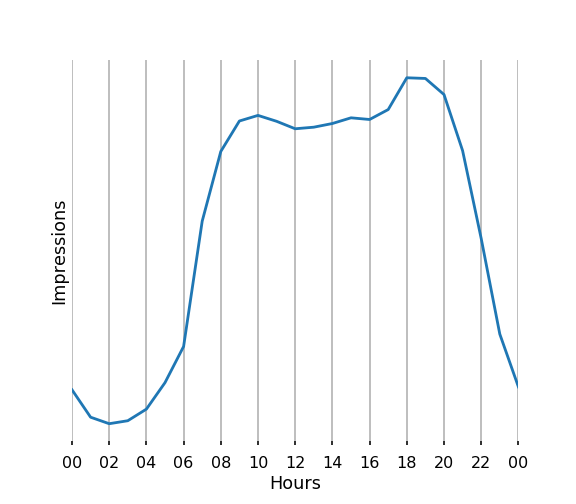
\includegraphics[width=12cm]{examples_day}
	\end{center}
	\vspace{-5mm}\caption{Пример показов рекламы за сутки}
	\label{fig:examples_day}
\end{figure}
 
\begin{figure}[!hhh]
	\begin{center}
		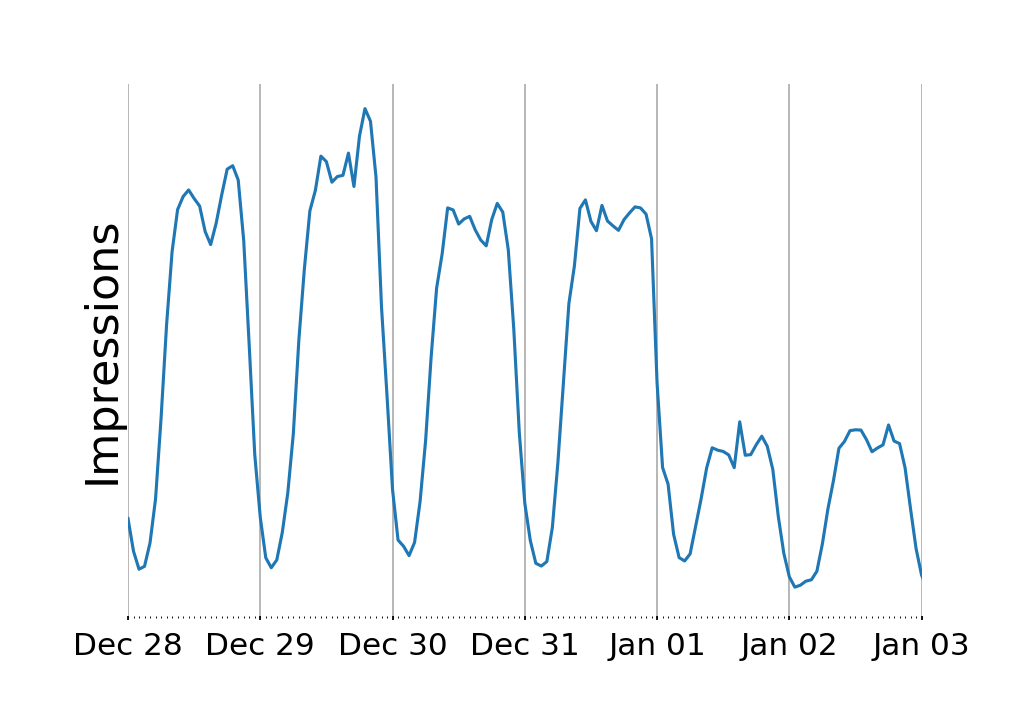
\includegraphics[width=12cm]{cp_mean_2}
	\end{center}
	\vspace{-5mm}\caption{Пример показов рекламы с разладкой за неделю}
	\label{fig:examples_month}
\end{figure}

Обозначим временной ряд $Y = (y_1, \dots, y_n)$. Наблюдаемые значения ряда можно представить в виде суммы компонент:
$$ Y = T + S + E $$, 
где  $ T = (t_1, \dots, t_n) $ компонента-тренд, $ S = (s_1, \dots, s_n) $ периодическая компонента, $ E = (\epsilon_1, \dots, \epsilon_n) $ остатки или шум.
Каждую из этих компонент требуется промоделировать. Это можно сделать, например, следующим образом:
$$ t_i = const, \quad \forall i \in (1, \dots, n) $$
$$ s_i = A \cos(\frac{2\pi}{a} i + \phi), \quad \forall i \in (1, \dots, n) .$$,
где $i$ индекс элемента ряда; $A$ --- амплитуда; $a$ --- период; $\phi$ --- фаза
$$ \epsilon_i \sim N(\mu, \sigma^2), \quad \forall i \in (1, \dots, n)  $$

Ряды, которые мы хотим смоделировать имеют мультипликативность (амплитуда колебаний меняется пропорционально изменению тренда). При моделировании, такого эффекта можно достичь взяв экспоненту от моделируемого ряда:
$$ Y^{(mult)} = e^{T + S + E} $$
\todo[inline]{С экспонентой решил переобозначить ряд как $Y^{(mult)} $, не уверен, что получилось изящно и корректно.}


Далее нам нужно промоделировать разладку. Конструируя модель разладки будем исходить из следующих предпосылок к свойствам разладки:
\begin{itemize}
	\item Разладка только в одной точке ряда
	\item Разладка только в тренде
	\item Разладка может отсутствовать с некоторой вероятностью $1 - \rho$
\end{itemize}
Формально это можно описать так: пусть $\tau$ --- точка (индекс) разладки, тогда тренд с разладкой будет иметь вид:
$$ \tilde{t_i} =
	\begin{cases}
		t_i, & i < \tau \\
		t_i + \delta, & i \geqslant \tau
	\end{cases}
$$
, где $ \delta $  --- значение разладки.

Тренд с разладкой тогда будет выглядеть следующим образом:

$$ \tilde{T} = (\tilde{t_1}, \dots, \tilde{t_n}) $$

Значение разладки является случайной величиной, которую можно моделировать по тому или иному закону. В данной работе мы будем моделировать значение разладки из нормального распределения, с некоторой вероятностью возникновения $ \rho $:

$$   
\delta = \begin{cases}
    		\delta^* \sim N(\mu^{(cp)}, \sigma^{2(cp)}), & \rho \\
  		0, & 1 - \rho
	\end{cases} 
$$

Таким образом, $\delta$ является случайной величиной с распределением-смесью и ее плотность распределения можно записать так:
$$ p(\delta) = \rho N(\mu^{(cp)}, \sigma^{2(cp)}) + (1-\rho) 0$$

\todo[inline]{Запись кажется не совсем корректной...}

При этом точка разладки  $\tau$ тоже является случайной величиной с равномерным распределением на $ [n_0, \dots, n ] $, где $ n_0 $ --- самая первая возможная точка разладки, которая задается параметром. $n_0$ введена намеренно, чтобы разладка при моделировании не возникала в первых точках ряда.

Таким образом, моделируемый ряд с разладкой будет иметь следующий вид:
$$ Y = e^{\tilde{T} + S + E}  $$

В результате модель временного ряда имеет пять параметров: $ A, a, \phi, \mu, \sigma $, а модель разладки имеет еще пять параметров: $ \delta, \mu^{(cp)}, \sigma^{(cp)}, \rho, n_0 $.

\section{Методы обнаружения разладки}


Опишем один из подходов к обнаружению разладки. Данный подход не является единственным, хотя заключает в себе широкое разнообразие методов. Как правило, у временного ряда есть некоторая структура (сигнал), которая может быть описана той или иной моделью. Идея подхода заключается в том, что около точки разладки модель плохо описывает временной ряд. Используя некоторую функцию ошибки мы можем измерять то, насколько хорошо или плохо описывает выбранная модель реальные данные в некотором диапазоне. 

Можно выделить два типа методов в данном подходе:
\begin{itemize}
	\item Методы на основе предсказания
	\item Методы на основе аппроксимации
\end{itemize}

Разберемся как работают методы на основе аппроксимации.

Пусть $l$ четное вещественное число, называемое длиной окна. При этом  $ 1 < l < n $. С помощью длины окна из исходного ряда образуется последовательность подрядов $W = \{ w_j \}_{j=1}^k$, где $k = n - l + 1$ --- количество таких подрядов; а $ w_j = (y_j, \dots, y_{j+l+1}) $ --- $j$-ый подряд. Каждый подряд  $w_j$  в свою очередь делится на два подряда одинаковой длины (это возможно поскольку $l$ четное по условию): $ W^{(left)} = \{w_j^{(left)} \}  =  (y_j, \dots, y_{\frac{j+l+1}{2}})$ и $W^{(right)} = \{w_j^{(right)} \} = (y_{\frac{j+l+1}{2}}, \dots, y_{j+l+1})$.

Таким образом, для каждого ряда $W$ можно сформировать тройки рядов: 
$$ W^{(all)} = \{w_j^{(all)} \}_{j=1}^k =  \{(w_j; w_j^{(left)}; w_j^{(right)}) \}_{j=1}^k  $$

Пусть есть функция ошибки $c(\cdot)$ , такая что:
$$c(x) = \min_{\theta}{\sum_{p=1}^m(x_p - f(x_p | \theta))^2 }$$
, где $x$ некоторый вещественный временной ряд длины $m$, а $f(x | \theta)$ некоторая модель этого временного ряда с параметрами $\theta$.

Функция $f(x|\theta)$ может быть линейной ($\theta = (const)$):
$$ f(x | const) = const $$
Либо другой подходящей под наш ряд функцией, например:
$$ f(x | A, a, \phi) = A\cos(\frac{2\pi}{a}x + \phi) $$.

Функция ошибки позволяет нам рассчитать насколько хорошо аппроксимируется отрезок ряда с помощью выбранной модели. Однако, для обнаружения самой разладки необходимо еще ввести функцию разладки:
$$ F(W^{(all)}) = \frac{c(W) - c(W^{(left)}) - c(W^{(right)})}{h} $$
, где $h$ --- значение нормировки.


Расчет нормы является открытой проблемой, поскольку имеются разные варианты её расчета со своими плюсами и минусами.
Например, можно рассчитывать её как значение функции ошибки на первом отрезке ряда (предполагая, что на этом отрезке не происходило разладок):
$$ h = f(w_1^{(all)}) = c(w_1) - c(w_1^{(left)}) - c(w_1^{(right)})  $$

Итого, взяв ряд $Y$ мы "скользим" по нему окном длины $l$ и рассчитываем значения функции разладки $F()$ для каждого из получаемых подрядов $W^{(all)}$. Функция разладки начинает расти в окрестности точки разладки $\tau$, следовательно можно задать некий порог $\alpha$. Такой что при превышении функции разладки этого порога в какой-то точке $\hat{\tau}$ можно считать, что разладка произошла в этой точке.

\section{Оценка качества}

В рамках данной работы мы разрабатываем систему своевременного оповещения о разладках во временных рядах. При такой постановке задачи важны две характеристики: точность обнаружения разладки и скорость обнаружения разладки. Поскольку мы используем моделированные данные, то мы точно знаем в каких из смоделированных нами рядов произошла разладка, а в каких разладки не было. Более того, мы точно знаем момент разладки. Благодаря этому мы можем строить матрицы сопряжённости и считать метрики качества. При этом надо понимать, что в такой постановке задачи нам важно обнаружить разладку не позднее какого-то срока, иначе оповещение о разладке будет несвоевременным. 

Разберем четыре возможных варианта:
\begin{itemize}
	\item Разладка произошла и метод обнаружил точку разладки \textbf{после} фактической точки, но не слишком поздно. Такая ситуация попадает под категорию True positive
	\item Разладка произошла и метод не обнаружил точку разладки, либо обнаружил её до фактической разладки, либо обнаружил её сильно после фактической разладки. False negative
	\item Разладки не было, но метод обнаружил разладку. False positive
	\item Разладки не было и метод не обнаружил разладку. True negative
\end{itemize}

Договорившись о таком способе оценки качества, можно строить ROC-кривые (изменяя порог $\alpha$) для разных методов обнаружения разладки и таким образом, сравнивая как работают те или иные методы в контролируемой среде эксперимента.

%В данной работе будут использоваться реальные данные компании, занимающейся рекламой в мобильных приложениях.
%На рисунке ~\ref{fig:1_initial} приведены данные о показах онлайн-рекламы по часам за 5 месяцев.
%
%\begin{figure}[!hhh]
%	\begin{center}
%		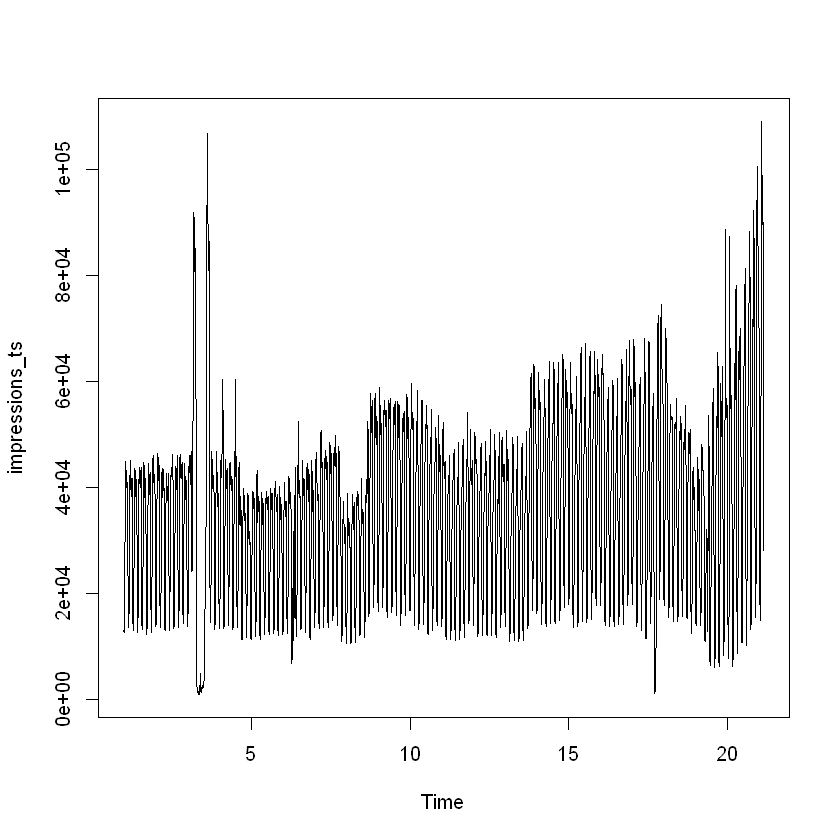
\includegraphics[width=12cm]{1_initial}
%	\end{center}
%	\vspace{-5mm}\caption{Исходные данные показов рекламы.}
%	\label{fig:1_initial}
%\end{figure}
%
%Для прогнозирования, независимо от метода, тем выше будет качество прогноза, чем качественнее исходный ряд, поэтому постараемся локализовать и устранить часть проблем. Очевидно в исходном ряду есть несколько проблем:
%
%\begin{itemize}
%	\item На графике видны явные выбросы --- резкие скачки или провалы значений. Выбросы связаны, как правило, с техническими неполадками, поэтому заменим их на средние соседние значения.
%	\item В первой половине временного ряда виден провал в данных в виде ступеньки и вскоре возврат к прежним значениям. Причиной этому являются технические неполадки, происходившие в этот период.
%\end{itemize}
%
%Суммарно в ряду были признаны аномальными 362 точки (что соответствует примерно 10\%). На рисунке ~\ref{fig:2_drop_na} изображен график с удаленными аномальными значениями. Заменим удаленные значения на среднее значение между аналогичным часом и днем недели прошлой и будущей недель (рисунок ~\ref{fig:3_fill_na}).
%
%\begin{figure}[!hhh]
%	\begin{center}
%		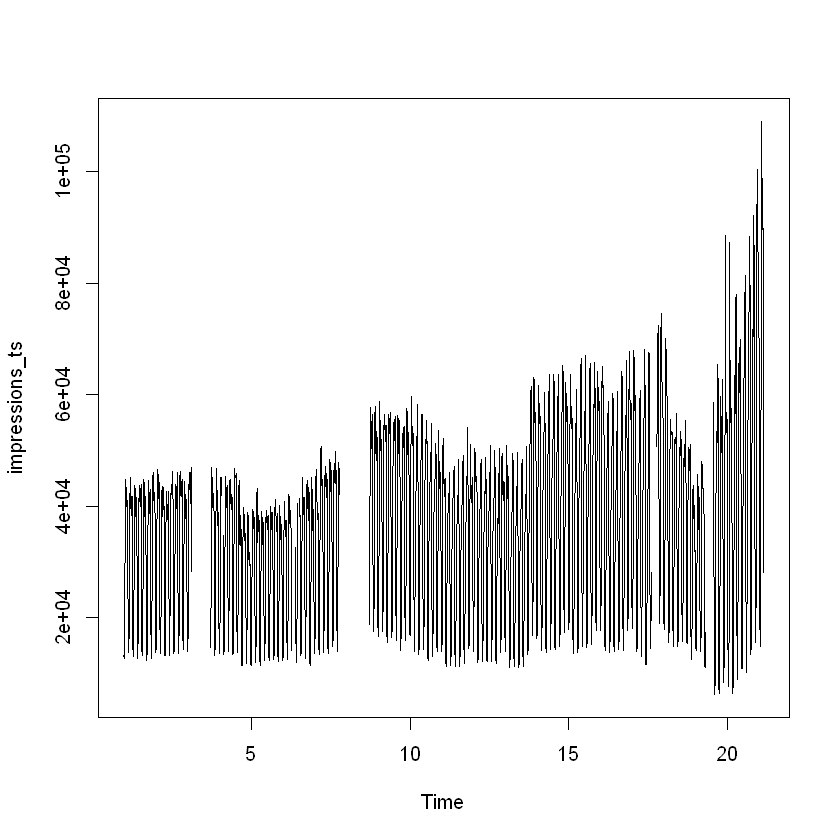
\includegraphics[width=12cm]{2_drop_na}
%	\end{center}
%	\vspace{-5mm}\caption{Данные показов рекламы после удаления аномальных точек.}
%	\label{fig:2_drop_na}
%\end{figure}
%
%\begin{figure}[!hhh]
%	\begin{center}
%		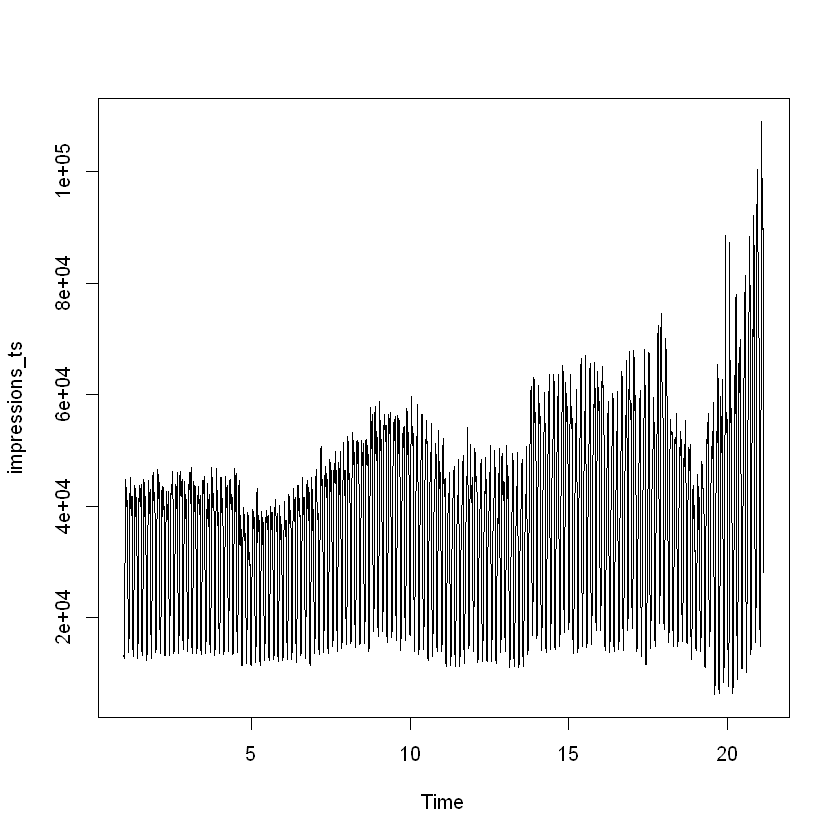
\includegraphics[width=12cm]{3_fill_na}
%	\end{center}
%	\vspace{-5mm}\caption{Показы рекламы после замены аномальных значений.}
%	\label{fig:3_fill_na}
%\end{figure}
%
%Далее необходимо произвести декомпозицию ряда на тренд, периодичную составляющую и остатки. Наибольшую сложность представляет выделение устойчивой периодичности, поэтому для этих целей необходимо изучить ряд внимательнее. Прежде всего, требуется определить какой характер имеет периодичность - аддитивный или мультипликативный (раздел ~\ref{sec:preprocessing}). Для этого извлечем тренд из ряда с помощью SSA с окном равным одной неделе (168 часов). Получившийся график остатков (рисунок ~\ref{fig:4_remove_trend}) не имеет сильно возрастающих колебаний, то есть явной мультипликативности в исходном ряде нет.
%
%\begin{figure}[!hhh]
%	\begin{center}
%		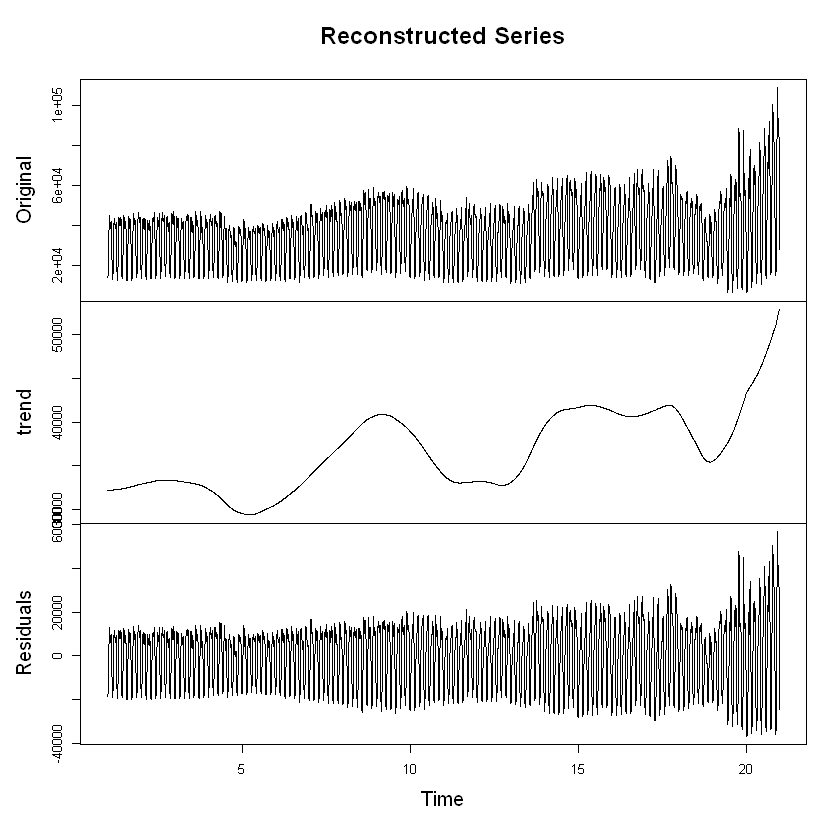
\includegraphics[width=12cm]{4_remove_trend}
%	\end{center}
%	\vspace{-5mm}\caption{Извлечение тренда из ряда с помощью SSA.}
%	\label{fig:4_remove_trend}
%\end{figure}
%
%Однако, если провести аналогичную процедуру для логарифма исходного ряда, то амплитуда колебаний графика остатков (после удаления тренда) больше похожа на одинаковую (рисунок ~\ref{fig:5_ln_remove_trend}).
%
%\begin{figure}[!hhh]
%	\begin{center}
%		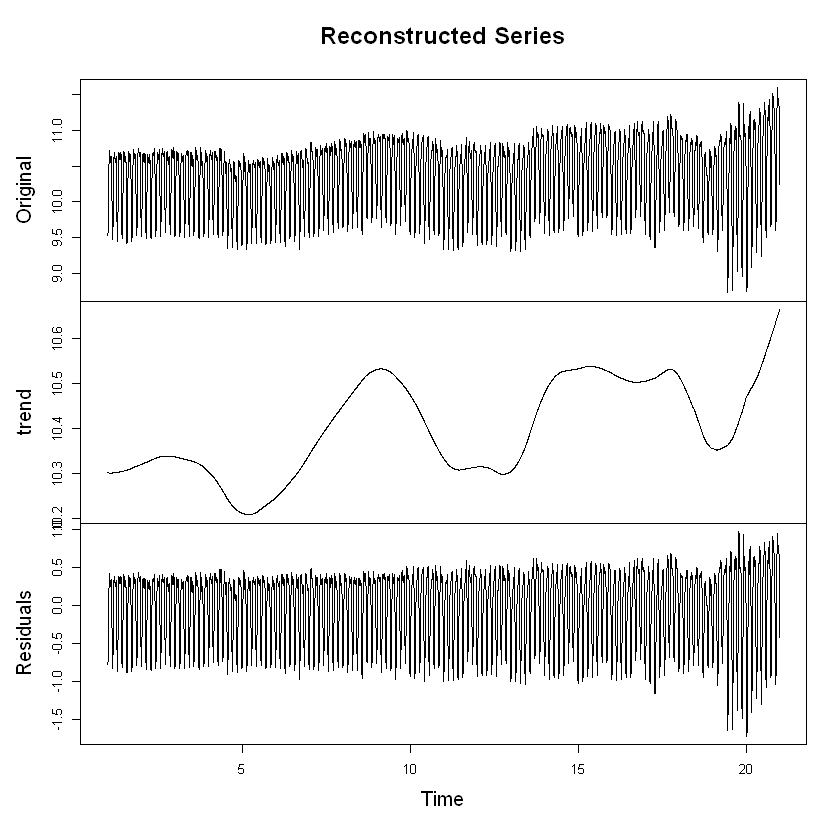
\includegraphics[width=12cm]{5_ln_remove_trend}
%	\end{center}
%	\vspace{-5mm}\caption{Извлечение тренда из логарифма ряда с помощью SSA.}
%	\label{fig:5_ln_remove_trend}
%\end{figure}
%
%Для подтверждения этой мысли построим огибающую кривую, описанную в первой главе (раздел ~\ref{sec:preprocessing}) для первого и второго случаев. Из графиков ~\ref{fig:6_envelope_curve} и ~\ref{fig:7_ln_envelope_curve} становится очевидным, что при логарифмировании амплитуда колебаний становится гораздо более ровной. Поэтому будем считать периодичность ряда мультипликативной, соответственно в дальнейшем работать с логарифмом исходного ряда.
%
%\begin{figure}[!hhh]
%	\begin{center}
%		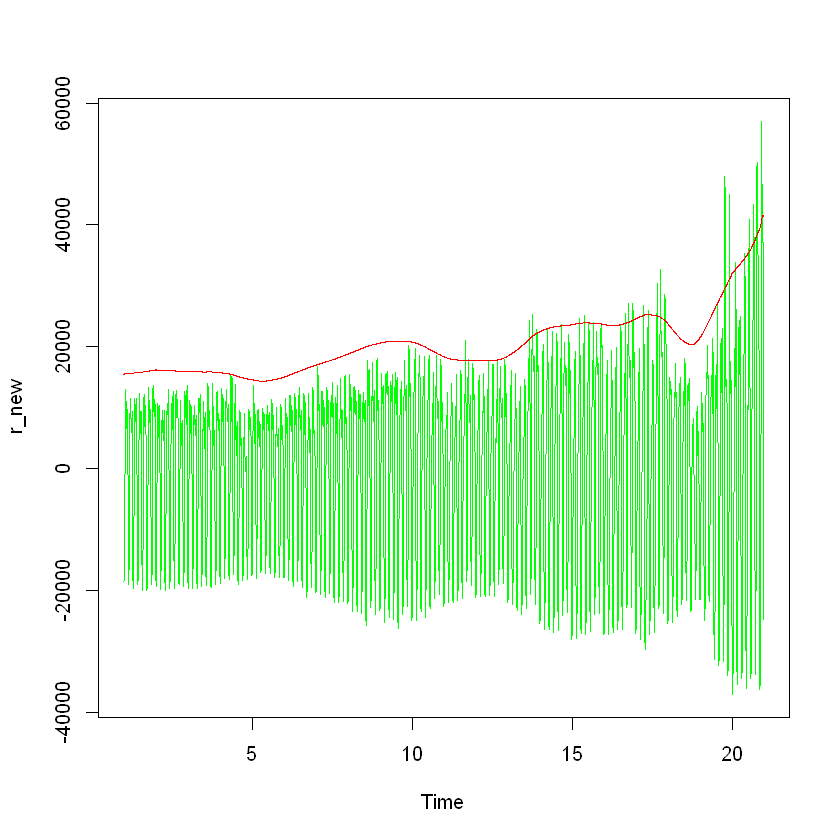
\includegraphics[width=12cm]{6_envelope_curve}
%	\end{center}
%	\vspace{-5mm}\caption{Окаймляющая кривая после извлечение тренда из исходного ряда.}
%	\label{fig:6_envelope_curve}
%\end{figure}
%
%\begin{figure}[!hhh]
%	\begin{center}
%		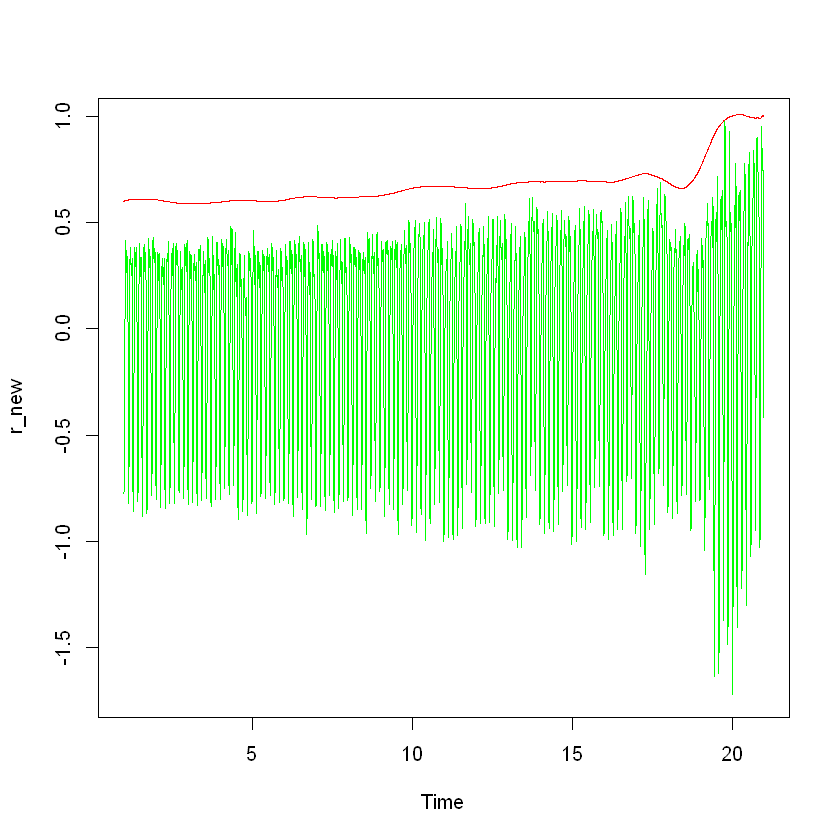
\includegraphics[width=12cm]{7_ln_envelope_curve}
%	\end{center}
%	\vspace{-5mm}\caption{Окаймляющая кривая после извлечение тренда из логарифма ряда.}
%	\label{fig:7_ln_envelope_curve}
%\end{figure}
%
%Теперь изучим ряд ближе с точки зрения ежедневной периодичности. После детального изучения был сделан вывод о том, что ряд следует разделить на три части --- первые 9 недель, последующие 8 недель и оставшиеся 3 недели.  Для демонстрации этого вывода построим несколько графиков периодичности (раздел ~\ref{sec:preprocessing}).
%
%Дело в том, что в первой части временного ряда ежедневная периодичность мало чем отличается друг от друга --- в этот период виден довольно устойчивый ежедневный паттерн (рисунок ~\ref{fig:8_ln_season_plot}). \\
%Во второй части видно явное различие между будними (рисунок ~\ref{fig:9_ln_season_plot_2}) и выходными днями (рисунок ~\ref{fig:10_ln_season_plot_3}). \\
%В последние 3 недели происходят зачастую хаотичные колебания в которых сложно уловить какой-либо паттерн (рисунок ~\ref{fig:11_ln_season_plot_4}). Далее вероятно потребуется рассматривать три данных отрезка ряда по отдельности.
%
%
%Итого, после первичной обработки ряд стал гораздо более гладким и однородным, было выяснено, что ряд имеет мультипликативную периодичность, а также было выяснено что ряд имеет разные паттерны периодичности на разных отрезках времени.
%
%
%\section{Сравнение различных моделей для прогнозирования показов рекламы}
%
%Попробуем подобрать модель, которая будет наилучшим образом прогнозировать выбранные данные на одни сутки. Выбирать будем из следующих моделей:
%\begin{itemize}
%	\item Базовая модель --- прогноз равен последнему известному дню.
%	\item SSA учитывающий все предыдущие значения с окном равным половине ряда
%	\item Скользящий SSA учитывающий определенное количество последних значений с окном равным половине ряда
%\end{itemize}
%
%Для сравнения моделей прогноз будет строиться не только на последние сутки, а скользящим способом на все предыдущие сутки в ряду.
%Обозначим весь временной ряд как вектор $ Y = y_1,...y_T $; часть временного ряда, на котором будет строиться модель, как $ \tilde{Y} = y_i,...,y_t $, где $ i \geq 1, t \leq T $; а прогноз,  как $ \hat Y = y_j,...y_h $, где $ h - j $ --- период на который строится прогноз, при этом $ h \leq t < T $. Таким образом, для каждого подхода мы будем строить $ m $ моделей и столько же прогнозов.
%Сравнивать результаты будем по показателю Average RMSE
%\[ Average  RMSE= \frac{\sum_{p=1}^m(\sqrt{\frac{\sum_{j=1}^h (y_j - \hat y_j)^2}{h}})}{m} \].
%
%В базовой модели нет никаких параметров, поэтому мы просто посчитаем показатель ошибки этой модели, и результаты приведем ниже в сравнении с другими моделями.
%Попробуем применить SSA для прогноза, для этого нам нужно решить следующие задачи:
%\begin{itemize}
%	\item Какое количество предыдущих значений учитывать при построении модели?
%	\begin{itemize}
%		\item Все доступные
%		\item Некоторое определенное количество
%	\end{itemize}
%	\item Какой размер окна выбирать на этапе разложения?
%	\begin{itemize}
%		\item „Стандартный“ равный половине ряда
%		\item Фиксированный
%	\end{itemize}
%	\item Какое количество троек выбрать на этапе разложения и как?
%	\begin{itemize}
%		\item Фиксированное количество первых троек
%	\end{itemize}
%	\item Учитывать ли специфику данного ряда, о которой писалось выше?
%	\begin{itemize}
%		\item Не учитывать
%		\item Учитывать и рассматривать каждый из этих рядов по отдельности
%	\end{itemize}
%\end{itemize}
%
%Попробуем задать некоторое количество параметров и для каждой комбинации параметров посчитать среднюю ошибку. Путем перебора оптимальным вариантом оказался прогноз с помощью модели с периодом (на котором строится модель) равным четырем неделям, длиной окна равной одной неделе и количеством собственных чисел равным пятидесяти. Сравнительные результаты приведены в таблице ~\ref{tab:compare_models}
%
%\begin{table}[!hhh]
%	\begin{center}
%		\begin{tabular}{rrrrrrrrrrrrr}
%			\hline
%			Тип модели & Период         & Длина окна  & Количество собственных троек & Средний RMSE \\
%			SSA        & 672            & 168         & 50                           & 2 754        \\
%			Базовая    &  -             &  -          &  -                           & 3 470        \\
%			SSA        & 672            & Стандартная & 50                           & 3 627        \\
%			SSA        & Весь доступный & 168         & 50                           & 3 996        \\
%			SSA        & Весь доступный & Стандартная & 50                           & 5 412        \\
%			SSA        & 168            & Стандартная & 5                            & 6 374        \\
%			\hline
%		\end{tabular}
%	\end{center}
%	\caption{Сравнительная характеристика моделей.}\label{tab:compare_models}
%\end{table}
%
%Примечательно, что прогноз с помощью такой модели оказался качественнее, чем прогноз с помощью базовой модели. Также стоит отметить, что прогноз с помощью SSA со стандартными параметрами показал результат значительно хуже.

% Заключение
% \input{concl}

\conclusion
%В данной работе были рассмотрены подходы к анализу временных рядов и метод анализа и прогнозирования SSA. Помимо этого описанные подходы были успешно применены к фактическим данным, были выявлены особенности и паттерны временного ряда, такие как мультипликативный характер ряда, ежедневная периодичность с отличиями в будние и праздничные дни. Более того, была проведена отдельная работа по поиску и замене аномальных значений. При этом методика прогнозирования, примененная в работе показала лучший результат в сравнении с базовым методом. В дальнейшем следует сравнить SSA с другими методами прогнозирования, продумать автономную методику первичного преобразования временного ряда, а так же опробовать полученные подходы к другим временным рядам.


% Не добавлять длинное тире в качестве разделителя
%\newcommand\BibDash{}
% Выделять курсивом
\let\BibEmph=\emph
\bibliographystyle{gost2008}

% Список литературы
% \bibliography{thesis}


\begin{thebibliography}{9}
	\bibitem{ssa_forecast} Голяндина Н.Э. Метод „Гусеница“-SSA: прогноз временных рядов. Учебное пособие. СПб., 2003.
	\bibitem{armstrong} Armstrong. Principles of Forecasting: A Handbook for Researchers and Practitioners. Kluwer Academic Publishers, 2001.
	\bibitem{dagum} Dagum, Estela, Bianconcini. Seasonal Adjustment Methods and Real Time Trend-Cycle Estimation, 2016.
	\bibitem{ssa_book} N. Golyandina, V. Nekrutkin, A. Zhigljavsky. Analysis of Time Series Structure - SSA and Related Techniques, 2001.
	\bibitem{hyndman} R. Hyndman, G. Athanasopoulos. Forecasting: Principles and Practice. 2013.
	\bibitem{moving_average} R. Hyndman. Moving averages. 2009.
	
\end{thebibliography}

% Приложения
\appendix
%\chapter{Графики периодичности}
%%\input{a}
%
%
%\begin{figure}[!hhh]
%	\begin{center}
%		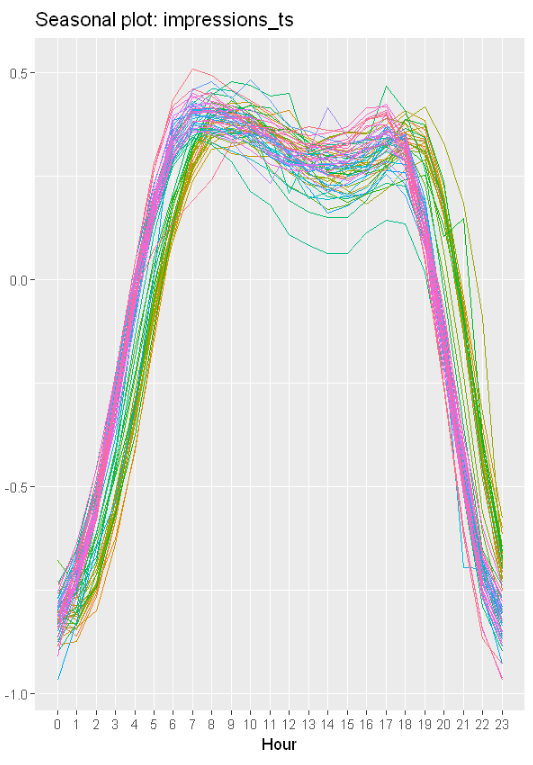
\includegraphics[width=12cm]{8_ln_season_plot}
%	\end{center}
%	\vspace{-5mm}\caption{График периодичности для первых девяти недель логарифма ряда.}
%	\label{fig:8_ln_season_plot}
%\end{figure}
%
%\begin{figure}[!hhh]
%	\begin{center}
%		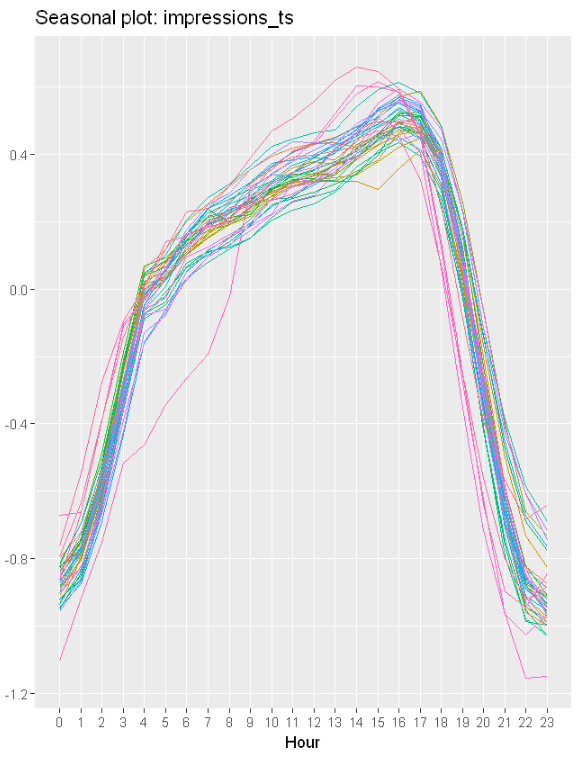
\includegraphics[width=12cm]{9_ln_season_plot_2}
%	\end{center}
%	\vspace{-5mm}\caption{График периодичности будних дней для недель с 10 по 18.}
%	\label{fig:9_ln_season_plot_2}
%\end{figure}
%
%\begin{figure}[!hhh]
%	\begin{center}
%		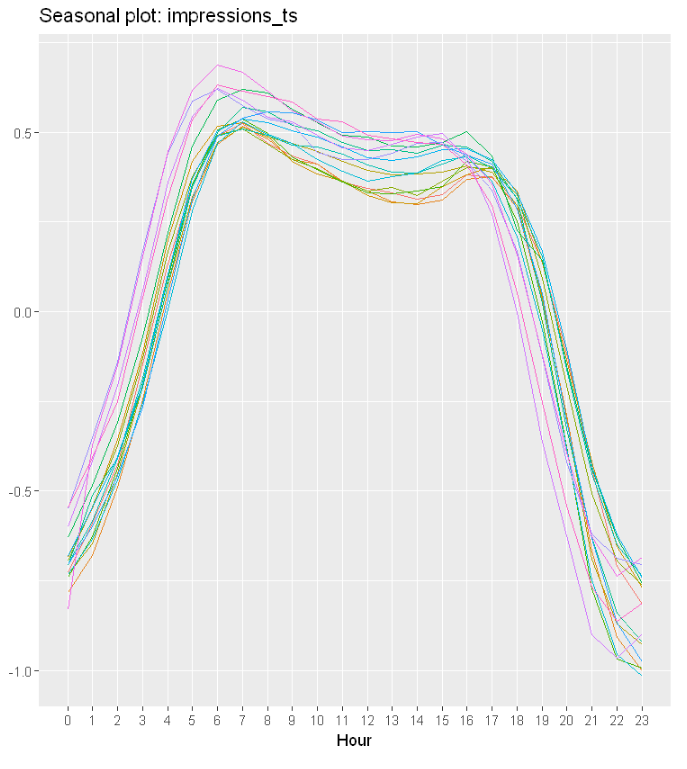
\includegraphics[width=12cm]{10_ln_season_plot_3}
%	\end{center}
%	\vspace{-5mm}\caption{График периодичности выходных дней для недель с 10 по 18.}
%	\label{fig:10_ln_season_plot_3}
%\end{figure}
%
%
%\begin{figure}[!hhh]
%	\begin{center}
%		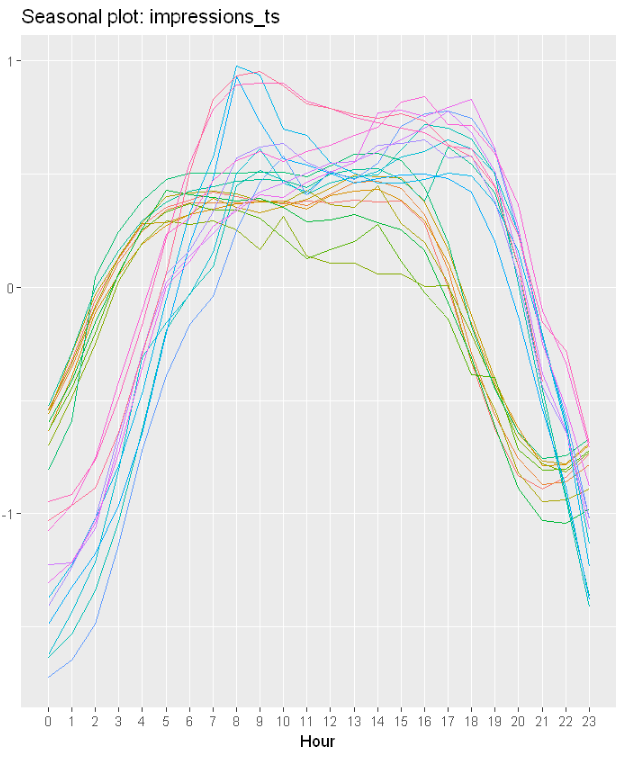
\includegraphics[width=12cm]{11_ln_season_plot_4}
%	\end{center}
%	\vspace{-5mm}\caption{График периодичности последних 3 недель.}
%	\label{fig:11_ln_season_plot_4}
%\end{figure}



\end{document}
